\documentclass[../Bachelorarbeit.tex]{subfiles}
\begin{document}
\chapter{Stand der Technik}
\label{chap:analyse}

Nachdem in Kapitel \ref{chap:einfuehrung} - \nameref{chap:einfuehrung} die ersten konkreten Überlegungen bis hin zu einem \nameref{sec:anwendungsszenario} aufgezeigt wurden um den Inhalt und die Funktionsweise des Prototypen zu umreißen, widmet sich dieses Kapitel der Domäne für die der Prototyp entwickelt wird.
Für diesen Zweck ist das Kapitel in zwei Abschnitte unterteilt. 
Im ersten Abschnitt (\nameref{chap:analyse:sec:sota}) wird ein Blick auf die Forschung und Fachliteratur geworfen, während sich der zweite Abschnitt (\nameref{chap:analyse:sec:analyBestehendeKonz}) mit echten Projekten beschäftigt, die eine Relevanz für den Prototypen darstellen.


\section{Literaturrecherche}
\label{chap:analyse:sec:sota}


\ideas{Einführung Themen aus der Entscheidungstheorie...Einzelne Punkte von Tufte, je nach Relevanz...Literaturrecherche ... sowie was aktueller Stand der Technik sowie Forschung.}



Daten OSM

\todoImprovement[]{weitere Analyse}
\todoInfo[]{Was ist gut, was ist schlecht?}

\section{Analyse von bestehenden Konzepten}
\label{chap:analyse:sec:analyBestehendeKonz}
\todoImprovement[]{Abschnittstitel konkretisieren}
\todoImprovement[]{Thema genauer ausarbeiten}


Webgis --> Browserbasiert 

\subsection{Google Maps}
\label{chap:analyse:sec:sota:sec:google_maps}
Google Maps\footnote{
	Google Maps ist unter der Adresse https://www.google.at/maps/ zu erreichen. Die getätigten Aussagen über die Webseite beziehen sich, wenn nicht anders erwähnt, auf den Stand von Sommer 2016.
} ist mit einer Milliarde User im Monat (Stand 2012) wahrscheinlich der verbreitete Online-Kartendienst im Internet (vgl. \cite{McClendonGoogleMapsBlog} und \cite{McClendonYoutube}).  
Neben der Routenplanung, mit Echtzeitdaten über das Verkehrsaufkommen, bietet Google Maps auch die Funktionalität IN DER NÄHE an.
Mit dieser Funktion lassen sich Orte anhand eines Suchbegriffes, wie beispielsweise Pizzeria, oder mittels vordefinierter Kategorien, wie zum Beispiel Restaurant, in der zuvor definierten Umgebung oder Stadt finden.


\subsection{Aufbau von Google Maps}
Die Darstellung von Google Maps ist optisch in zwei Teile unterteilt.
Zum einen die ausblendbare linke Seite, welche in die Bereiche \nameref{gmapsSearch} sowie die \nameref{gmapsList} der Ergebnisse und zum anderen der größere rechte Teil, mit der\nameref{gmapsMap} (siehe Abb.: \ref{fig:googlemapOverview} - \nameref{fig:googlemapOverview}).
Durch die blaue Hintergrundfarbe wird das \nameref{gmapsSearch} optisch von der \nameref{gmapsList} der Ergebnisse abgegrenzt.


\paragraph{Suchfeld}
\label{gmapsSearch}
Die Ansicht des Bereichs \nameref{gmapsSearch} kann der Abb.: \ref{fig:googlemapOverview} - \nameref{fig:googlemapOverview} entnommen werden und wird durch den roten Rahmen mit der Nummerierung 1 markiert (links oben).
Das Suchfeld stellt das zentrale Auswahlelement in Google Maps da. 
Neben dem eigentlich Textfeld, wurde an dieser Stelle auch ein Button integriert, mit dessen Hilfe ein weiteres Menü erscheint. 
Dieses Menü wird verwendet, um weitere Informationen  in der Karte ein- oder auszublenden, wie Beispielsweise die aktuelle Verkehrslage, oder allgemeine Optionen von Google Maps anzupassen wie unter anderem die Sprache.
Bei der eigentlichen Interaktion mit dem Suchfeld steht eine Unterstützung in Form einer Textvervollständigung zu Verfügung. 

\paragraph{Listendarstellung}
\label{gmapsList}
\nameref{fig:googlemapOverview} entnommen werden und wird durch den roten Rahmen mit der Nummerierung 2 markiert (links).
Dieser Bereich wird für die Darstellung der Suchergebnisse verwendet, welcher Anhand der Bewertungen gefiltert werden kann.
Jedes Ergebnis wird hier klar durch einen horizontalen Strich abgegrenzt.
Neben dem Namen und der Straße des Eintrages werden ein Bild, die durchschnittliche Bewertung sowie die Öffnungszeiten dargestellt, vorausgesetzt die Informationen sind vorhanden.

\paragraph{Kartendarstellung}
\label{gmapsMap}

\begin{figure}[H]
\centering
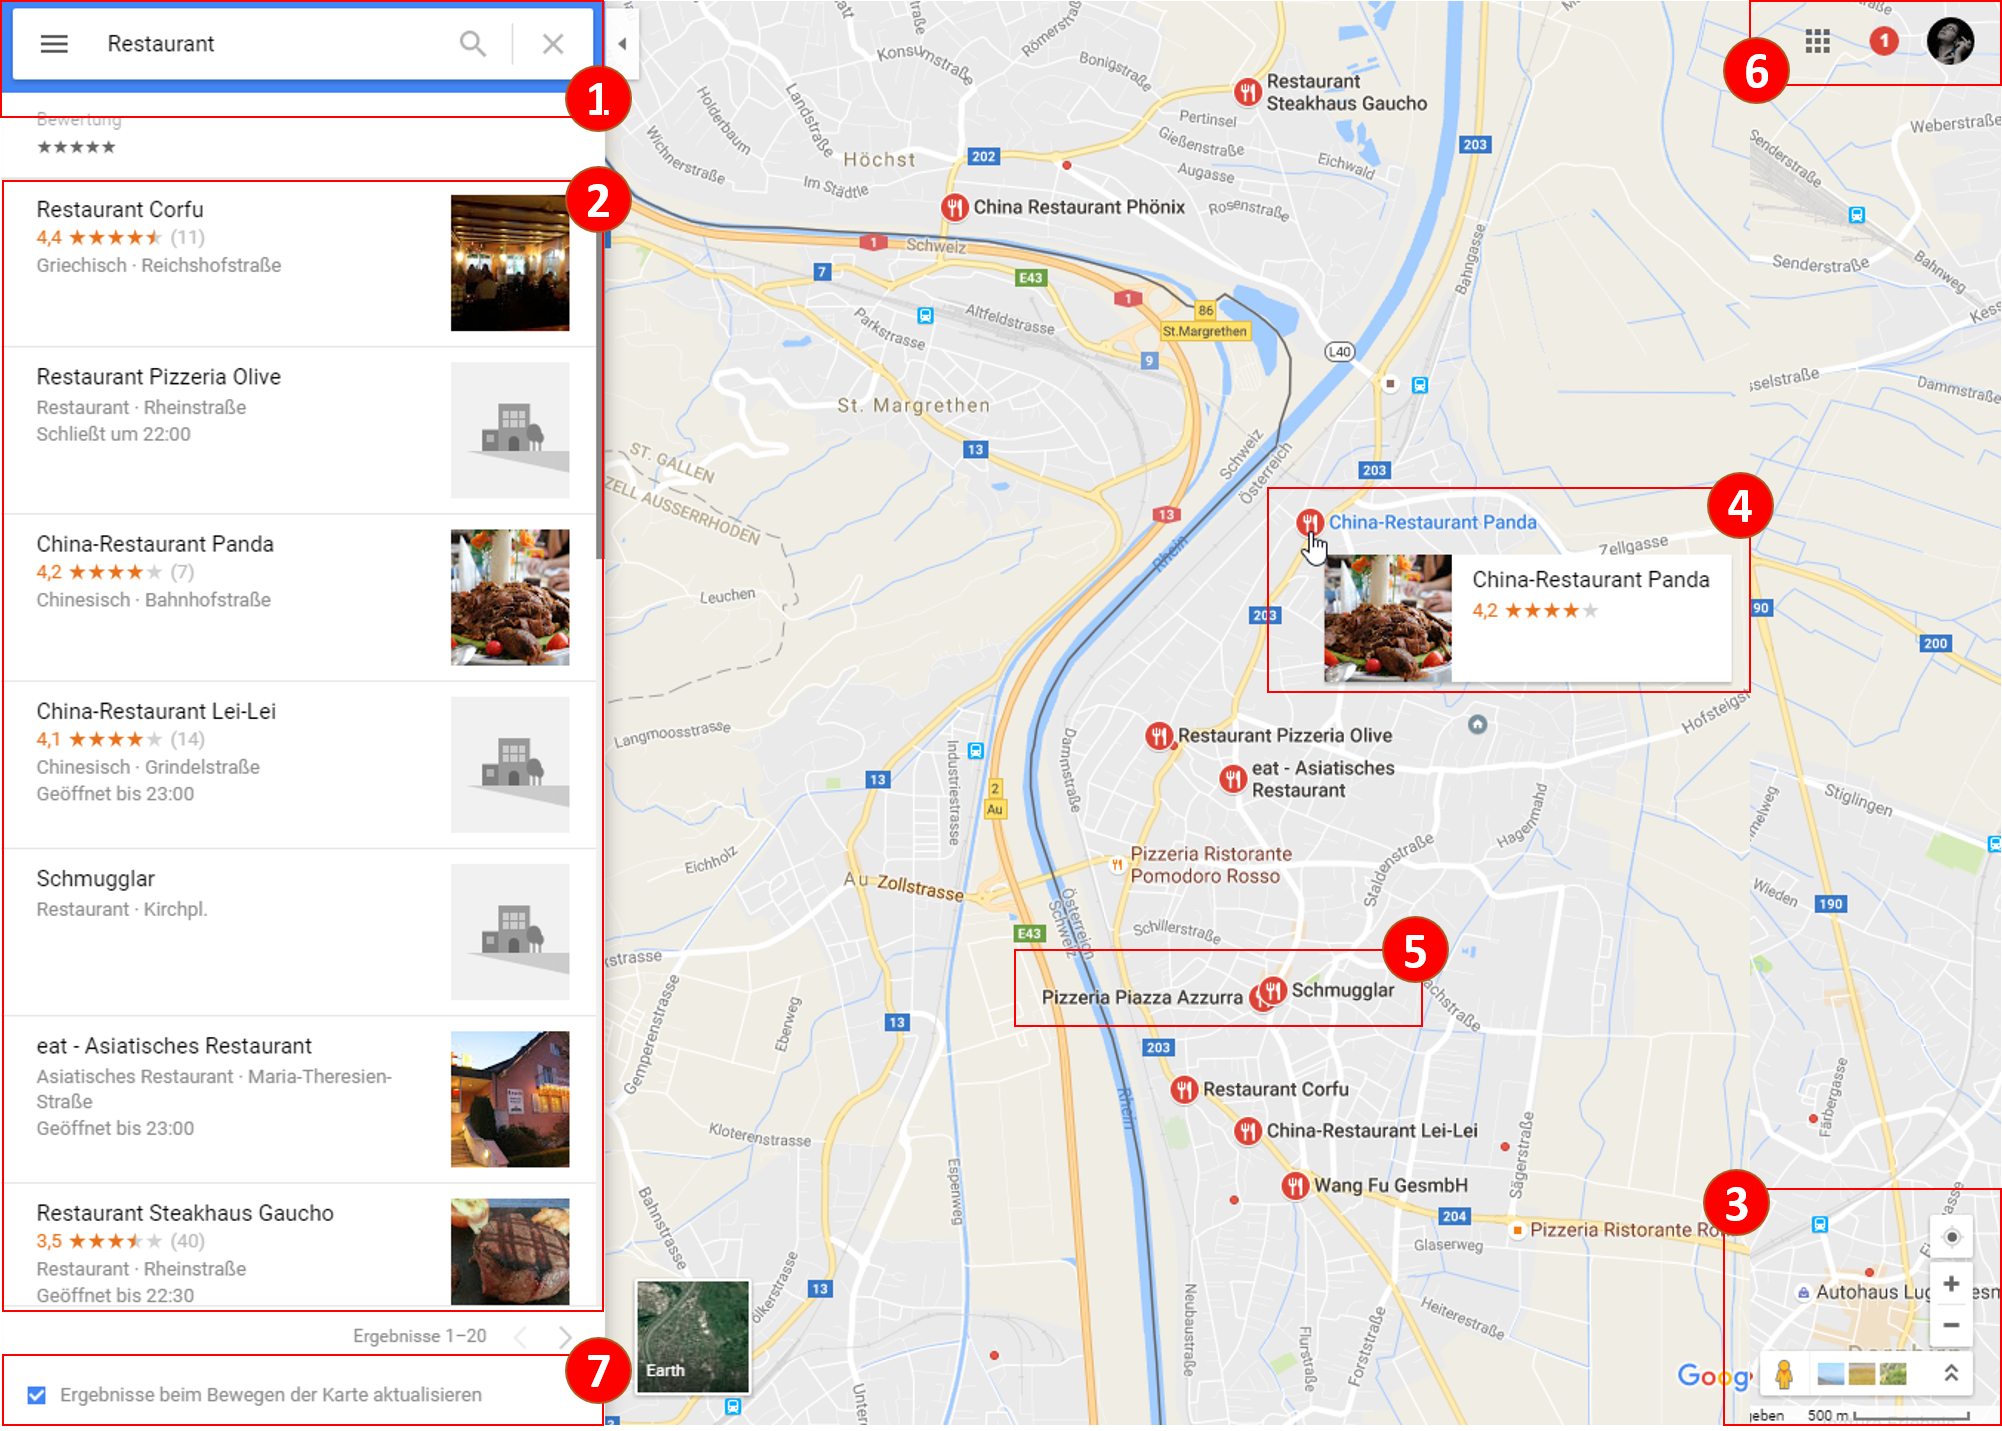
\includegraphics[width=1\linewidth]{img/StandDerTechnik/googlemapOverview}
\caption[Übersicht: Aufbau von Google Maps]{Übersicht: Aufbau von Google Maps. Bei der Abb. handelt es sich um eine bearbeitet Version des Screenshots. Aus Gründen der Übersichtlichkeit wurde ein Teil der Kartenbereichs entfernt (Quelle: eigene Ausarbeitung | Daten und Kartenmaterial: https://www.google.at/maps/ - Stand Sommer 2016)}
\label{fig:googlemapOverview}
\end{figure}



\subsection{Zusammenfassung Google Maps}

\begin{figure}[H]
\centering
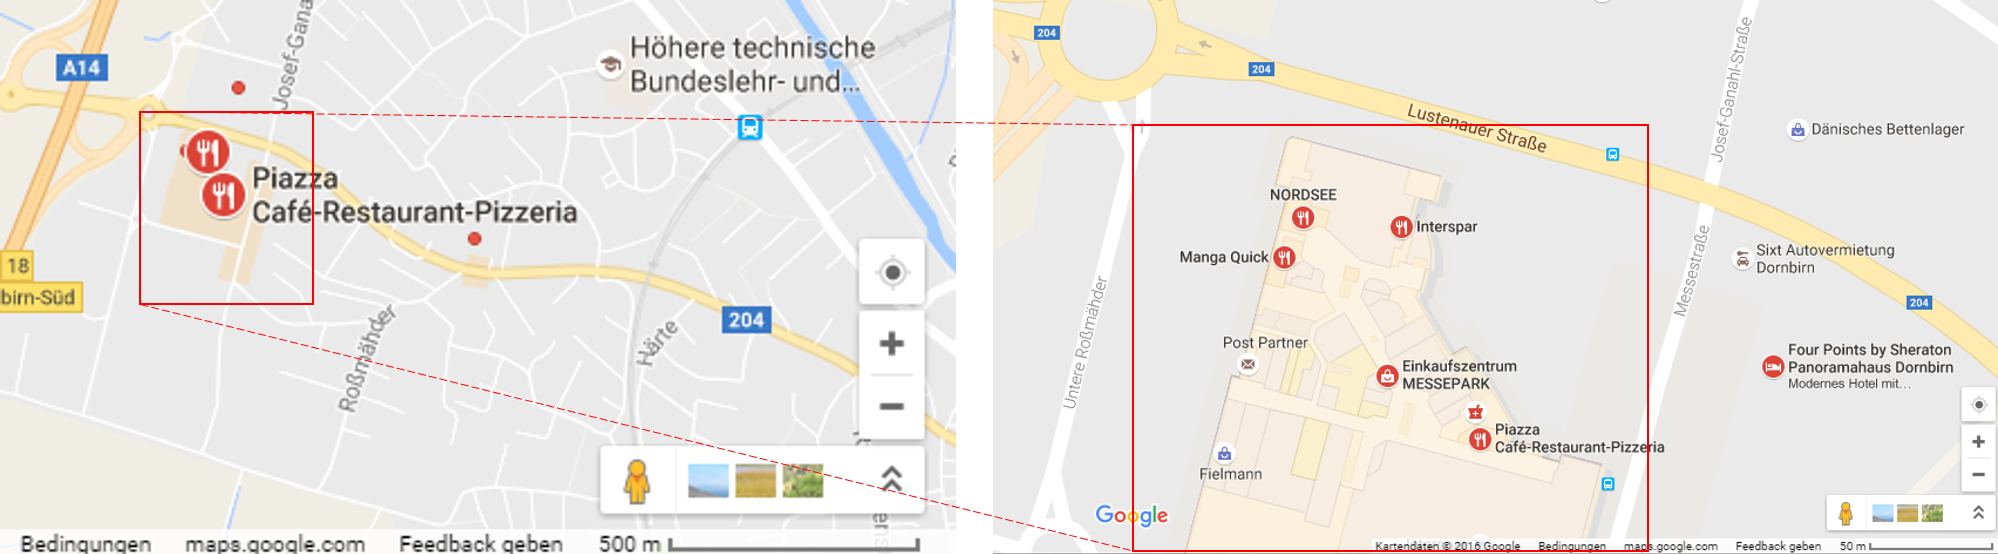
\includegraphics[width=1\linewidth]{img/StandDerTechnik/googlemapDetail}
\caption[Details: Überlagerung von Markierungen auf Google Maps]{Details: Überlagerung von Markierungen auf Google Maps. Der linke Kartenausschnitt zeigt eine Vergrößerung um den Faktor Zehn gegenüber dem rechten Kartenausschnitt. Der rote Rahmen markiert das jeweils das gleiche Gebäude. (Quelle: eigene Ausarbeitung | Daten und Kartenmaterial: https://www.google.at/maps/ - Stand Sommer 2016)}
\label{fig:googlemapDetail}
\end{figure}


Füge einen fehlenden Ort hinzu

\subsection{Airbnb}
Bei Airbnb handelt es sich um eine Webseite die sich auf die Vermittlung von Unterkünften spezialisiert hat\footnote{
	Google Maps ist unter der Adresse https://www.google.at/maps/ zu erreichen. Die getätigten Aussagen über die Webseite beziehen sich, wenn nicht anders erwähnt, auf den Stand von Sommer 2016.
	}. 
Dabei können sich gastgebende Personen registrieren und Übernachtungsmöglichkeiten von einem Zimmer bis hin zu ganzen Immobilien anbieten. 
Anhand diverser Such- und Filterkriterien ermöglicht die Webseite den Suchenden eine passende Unterkunft zu suchen und diese über die Webseite zu reservieren.
Neben klassischen Bewertungen bietet die Webseite auch Social Media Komponenten wie Profile, das hochladen eigener Fotos und das liken  sowie die Möglichkeit sich als gastgebende Person eine eigene Marke aufzubauen (vgl. \cite{Yannopoulou2013}, S. 3).

\subsubsection*{Aufbau von Airbnb}
Nachdem auf der Startseite die gewünschte Stadt in der man übernachten möchte, sowie optional das Start- und das Enddatum, ausgewählt wurden wird man auf die eigentliche Seite zur Planung weitergeleitet (siehe Abb.: \ref{fig:airbnbOverview} - \nameref{fig:airbnbOverview}).
Die Planungsansicht unterteilt sich in die drei Bereiche \nameref{airbnb:filter}, \nameref{airbnb:gridview} sowie der \nameref{airbnb:map}.
Die jeweiligen Bereiche sind durch unterschiedliche Farbgebungen des Hintergrundes klar voneinander abgetrennt.

\paragraph{Auswahlkriterien/Filter}
\label{airbnb:filter}
Die Ansicht des Bereichs \nameref{airbnb:filter} kann der Abb.: \ref{fig:airbnbOverview} - \nameref{fig:airbnbOverview} entnommen werden und wird durch den roten Rahmen mit der Nummerierung 1 markiert (links oben).
Durch Änderungen in diesem Bereich werden die beiden anderen Bereiche (\nameref{airbnb:gridview} und \nameref{airbnb:map}) automatisch aktualisiert. 
Dieser Bereich ist in der Standardansicht in vier Zeilen aufgeteilt. 
In der ersten Zeile (ganz oben) befindet sich ein Textfeld welches Standardmäßig die zuvor ausgewählte Stadt/Region anzeigt. 
Sobald man das schreiben im Textfeld beginnt, wird man bei der Eingabe durch eine Auswahl passender Einträge unterstützt, welche unter dem Textfeld eingeblendet werden.
Mithilfe der zweiten Zeile von oben lassen sich die optionalen Daten von der Startseite (Start-, Enddatum und Anzahl der Gäste) nachtragen oder ändern.
Die Art der Unterkunft wird mit Hilfe der dritten Zeile von oben ausgewählt.\\
\\
In der vierten Zeile von oben werden die Preise mit Hilfe eines stilistischen Balkendiagramms angezeigt. Dabei verlaufen die Preise ansteigend auf der X-Achse.
Die Information über die Anzahl der Unterkünfte in der entsprechenden Preisklasse wird mithilfe der Y-Achse schematisch dargestellt
\footnote{Die genau Information kann aufgrund der fehlenden Beschriftung der Y-Achse oder einer anderen visuellen Unterstützung nicht abgelesen werden.
	}.
Mithilfe von zwei Schiebereglern kann die untere- und obere Grenze für die Preisspanne festgelegt werden, der jeweilige Betrag wird direkt unter den Reglern dargestellt.
Zusätzlich wird der durchschnittliche Preis der Region/Stadt unter der Preisspanne dargestellt.\\
\\
Mit einem klick auf den Button Filter (siehe Abb.: \ref{fig:airbnbOverview} - linke Seite zwischen oberen- und unteren roten Rahmen) wird der Bereich \nameref{airbnb:filter} expandiert und überlagert die  \nameref{airbnb:gridview}.
Dabei ist aufgefallen das die Platzierung des Buttons für mich etwas irritierend wirkt. 
Wie zuvor erwähnt, werden die einzelnen Bereiche durch die unterschiedliche Farbgebung des Hintergrundes abgegrenzt. 
Dabei befindet sich der Button Filter im grauen Bereich (\nameref{airbnb:gridview}) wenn man allerdings darauf klickt wird der expandierte Bereich in der hellen Hintergrundfarbe des \nameref{airbnb:filter}-Bereichs dargestellt.


\paragraph{Rasterdarstellung}
\label{airbnb:gridview}
Die Ansicht des Bereichs \nameref{airbnb:gridview} kann der Abb.: \ref{fig:airbnbOverview} - \nameref{fig:airbnbOverview} entnommen werden und wird durch den roten Rahmen mit der Nummerierung 2 markiert (links unten).
Die Ergebnisse der Einstellungen, welche im Bereich \nameref{airbnb:filter} getroffen wurden, werden hier in Form von Kacheln in einer Rasteransicht dargestellt.
Dies ist der einzige Bereich der über eine Scroll - Funktionalität verfügt.
Den Hintergrund von jedem Ergebnis stellt ein Bild der Unterkunft da. 
Durch die eingeblendeten Steuerelement
	\footnote{Die Steuerelemente werden eingeblendet sobald man mit dem Cursor über das Bild geht.} 
kann das Hintergrundbild durch andere Bilder aus der jeweiligen Galerie ersetzt werden. 
Des Weiteren werden neben dem Preis und des Profilbildes der gastgebenden Person auch die zusammengefassten Informationen der Unterkunft dargestellt. 
Mit einem klick auf Bild öffnet sich die entsprechende Detailseite der Unterkunft. 

\paragraph{Kartendarstellung}
\label{airbnb:map}
Die Ansicht des Bereichs \nameref{airbnb:map} kann der Abb.: \ref{fig:airbnbOverview} - \nameref{fig:airbnbOverview} entnommen werden und wird durch den roten Rahmen mit der Nummerierung 3 markiert (rechts).
Dieser Bereich unterstützt die Anwenderinnen bei der geografischen Orientierung dadurch, das die gleichen Ergebnisse wie im Bereich \nameref{airbnb:gridview} auf einer Karte visualisiert werden.
Dabei wird jede Unterkunft als eine eigenständige Markierung dargestellt, welche mit dem jeweiligen Preis versehen ist.
Durch einen klick auf die Markierung öffnet sich ein Popup, in welchem ein Bild der Unterkunft
\footnote{
	Auch hier gibt es im Popup die Möglichkeit sich durch die Galerie zu bewegen (siehe Absatz: \nameref{airbnb:gridview}).
	} 
sowie der Preis und weitere Informationen dargestellt werden. 
Wie auch im Absatz \nameref{airbnb:gridview} beschrieben lässt sich die Detailseite der Unterkunft über einen klick auf das Bild öffnen.
Eine Farbcodierung von Informationen ist dabei nicht angedacht, alle Markierungen sind gleich eingefärbt.
Allerdings wechselt eine Markierung die Farbe (von rot nach grau) sobald man auf ihn geklickt hat und das erscheinende Popup wieder schließt.
Markierungen sich auf Grund der Zoomstufe überlagern werden nicht gesondert dargestellt.

\begin{figure}[H]
	\centering
	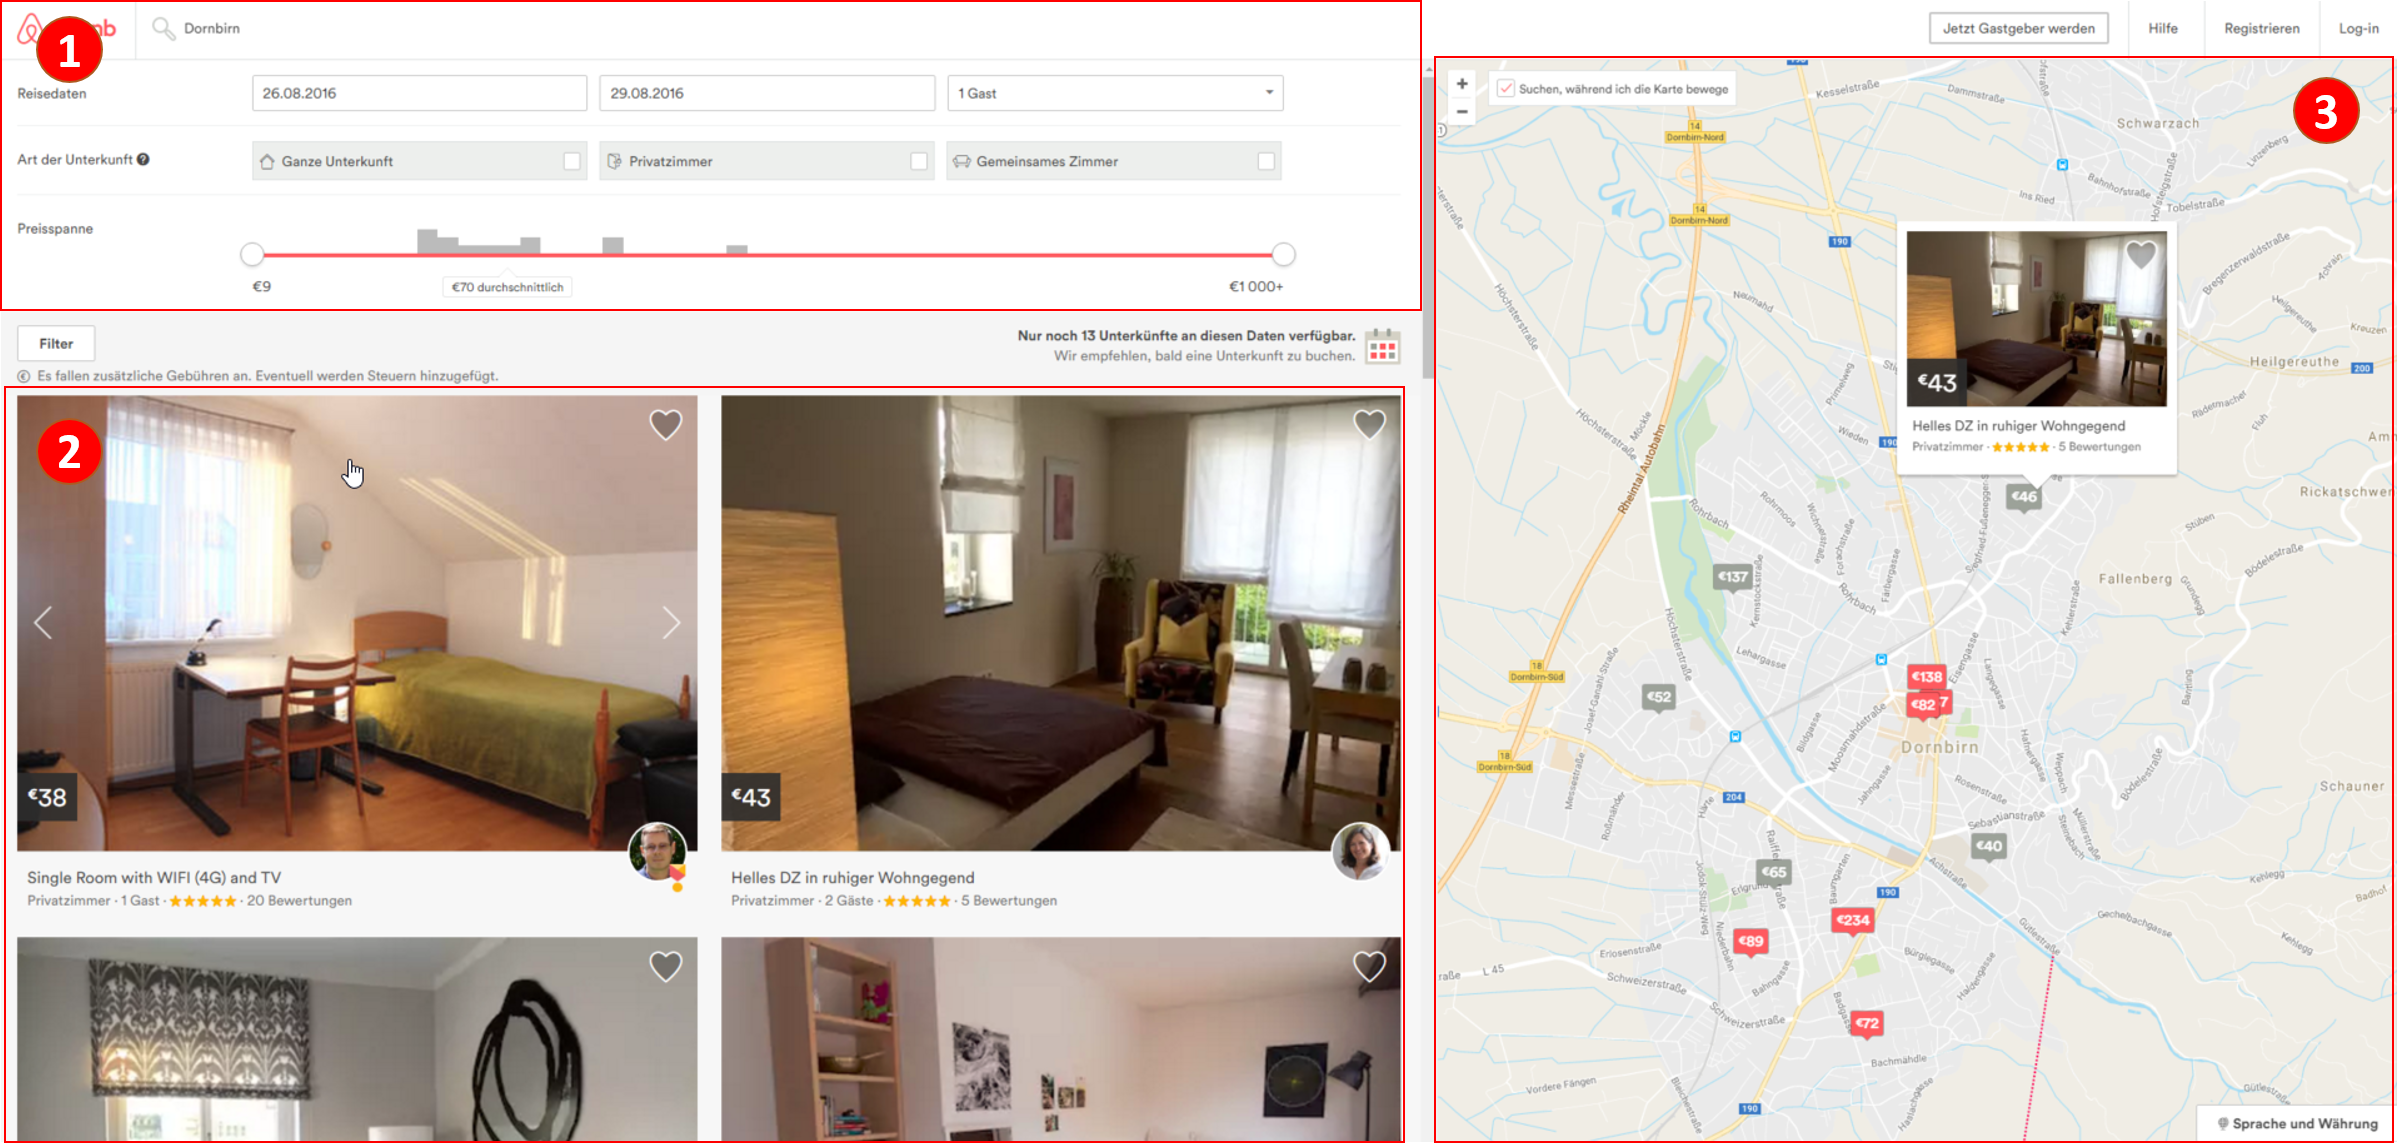
\includegraphics[width=1\linewidth]{img/StandDerTechnik/airbnbOverview}
	\caption[Übersicht: Aufbau von Airbnb]{Übersicht: Aufbau von Airbnb (Quelle: eigene Ausarbeitung | Daten und Kartenmaterial: https://www.airbnb.com/ - Stand Sommer 2016)}
	\label{fig:airbnbOverview}
\end{figure}

\subsubsection{Zusammenfassung Airbnb}
\label{airbnb:review}
Die Auswahlseite ist schlicht und übersichtlich gehalten wodurch die einzelnen Bereiche schnell identifiziert werden können, mit Ausnahme des Filter-Buttons (siehe Absatz: \nameref{airbnb:filter}). 
Die Funktionalität des Preisspannen Filters ist aus meiner Sicht sofort erkenntlich gewesen und bietet auf den ersten Blick eine gute Übersicht über die Preisverteilung der Unterkünfte.
Etwas unübersichtlich ist die \nameref{airbnb:map}, sobald mehrere Markierungen nebeneinander liegen wodurch diese (abhängig von der Zoomstufe) überlagert werden und der beschriftete Preis nicht mehr ersichtlich ist. \\
\\
Sehr interessant ist die Idee, die Ergebnisse auf zwei verschiedene Arten zu visualisieren (die Bereiche \nameref{airbnb:gridview} und \nameref{airbnb:map}).
Dies ermöglicht eine Auswahl nach der geografischen Lage (\nameref{airbnb:map}) sowie nach den Bilder der Unterkunft beziehungsweise den weiteren Informationen in der \nameref{airbnb:gridview}
Zusätzlich wurden die beiden Bereiche miteinander verknüpft. 
Sobald man mit der Maus ein Bild in der \nameref{airbnb:gridview} berührt wird die zugehörige Markierung auf der Karte dunkelgrün hervorgehoben (siehe Abb.: \ref*{fig:airbnbDetail} - \nameref{fig:airbnbDetail}) wodurch das abwechselnde Arbeiten in beiden Bereichen vereinfacht wird.


\begin{figure}[H]
\centering
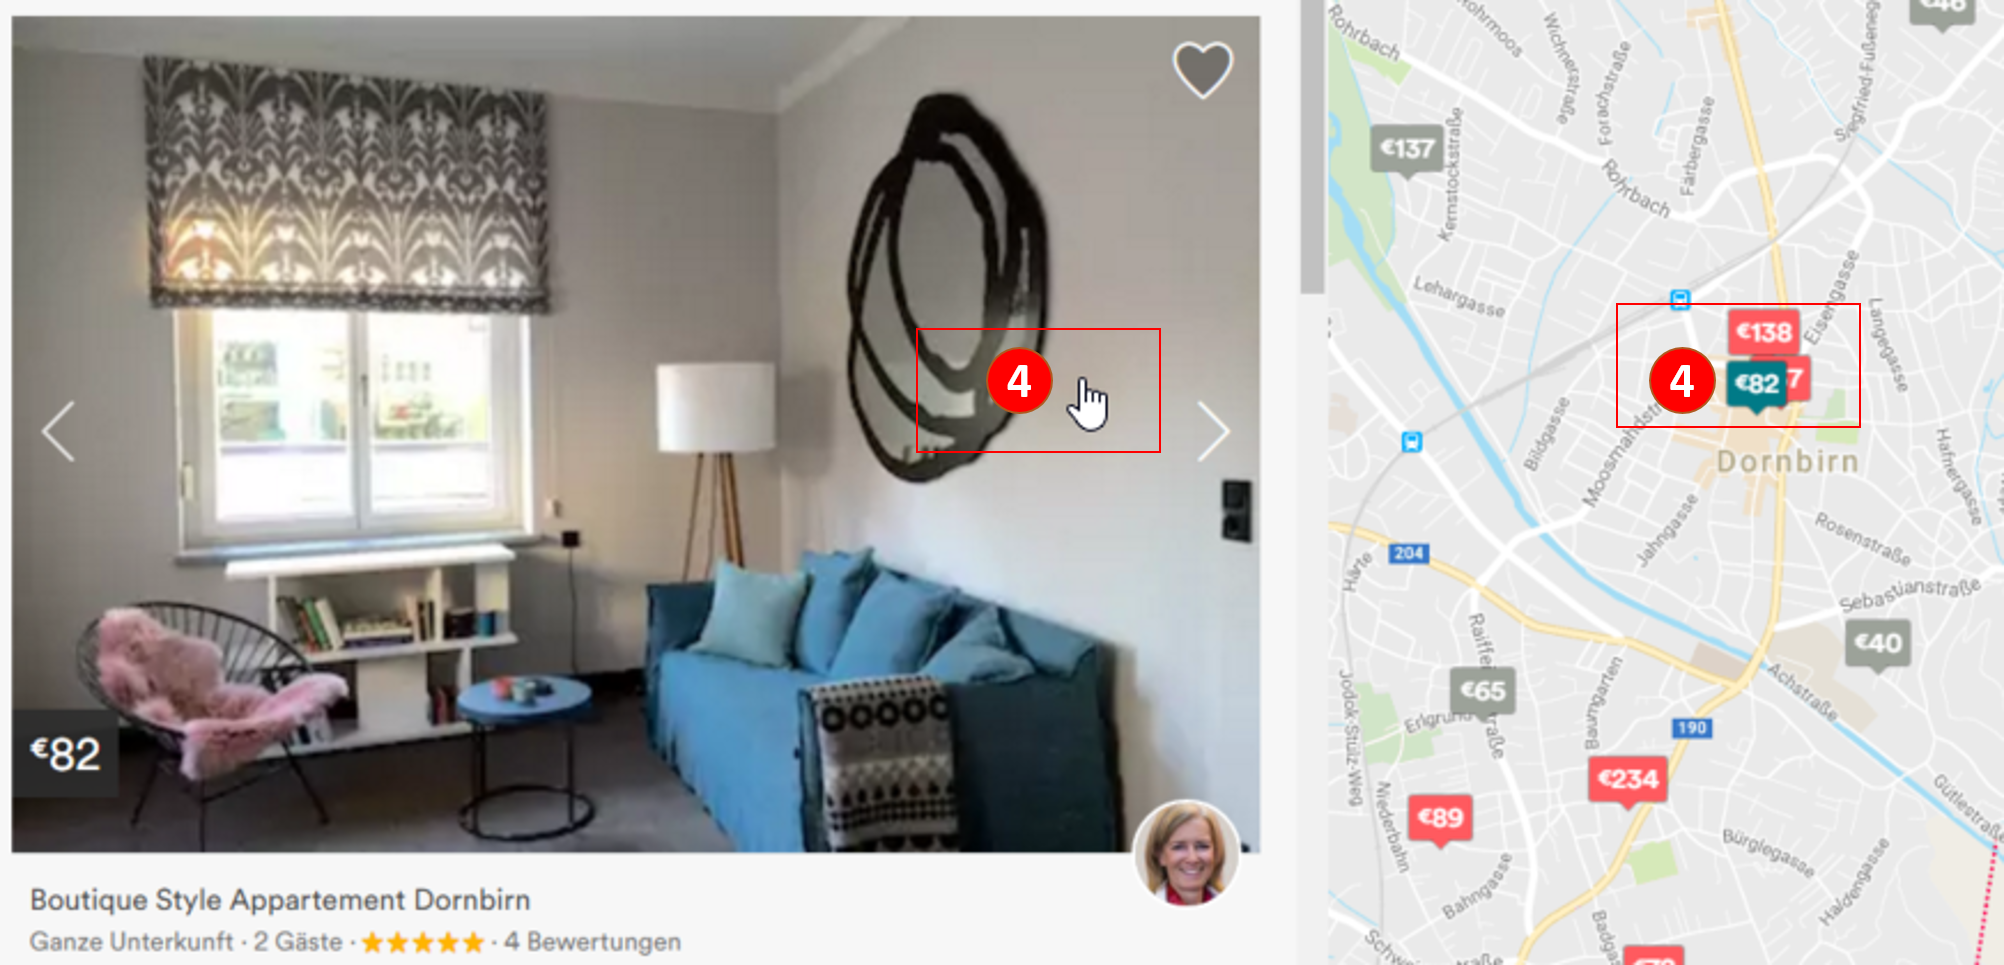
\includegraphics[width=1\linewidth]{img/StandDerTechnik/airbnbDetail}
\caption[Verknüpfung der Raster- und Kartenansicht]{Verknüpfung der Raster- und Kartenansicht (Quelle: eigene Ausarbeitung | Daten und Kartenmaterial: https://www.airbnb.com/ - Stand Sommer 2016)}
\label{fig:airbnbDetail}
\end{figure}




\subsection{Flightradar24}

\end{document}